
\section{Analysis}

% bring up features from #Background
% features:

\subsection{Experiment Setup}

Each device in the testbed has at least three active ethernet links:
One connecting it to a management server, and two connected to the
corresponding \Ac{dut} or loadgen (load generator). The management
server (kauas) uses pos tools to set boot images, boot, run setup and
testing scripts on the testbed devices and collect script output and
artifact files containing test results.

As figure \ref{setup} shows, each test contains two
devices. The \Ac{dut}, running \Ac{vpp}, and the loadgen, generating
packets and sending them to the \Ac{dut} to test \Ac{vpp}. \Ac{vpp}
then forwards the packets back to the loadgen which allows the loadgen
to create accurate throughput and latency measurments.

On the \Ac{dut} some debug information like error counts are beeing
gathered from the \Ac{vpp} CLI interface and Linux perf tools
\cite{perf} attach to the vpp process to collect time spent per symbol
and stats like cpu cycles or cache misses.

\begin{figure}[!ht]
\noindent\hspace{0.5mm}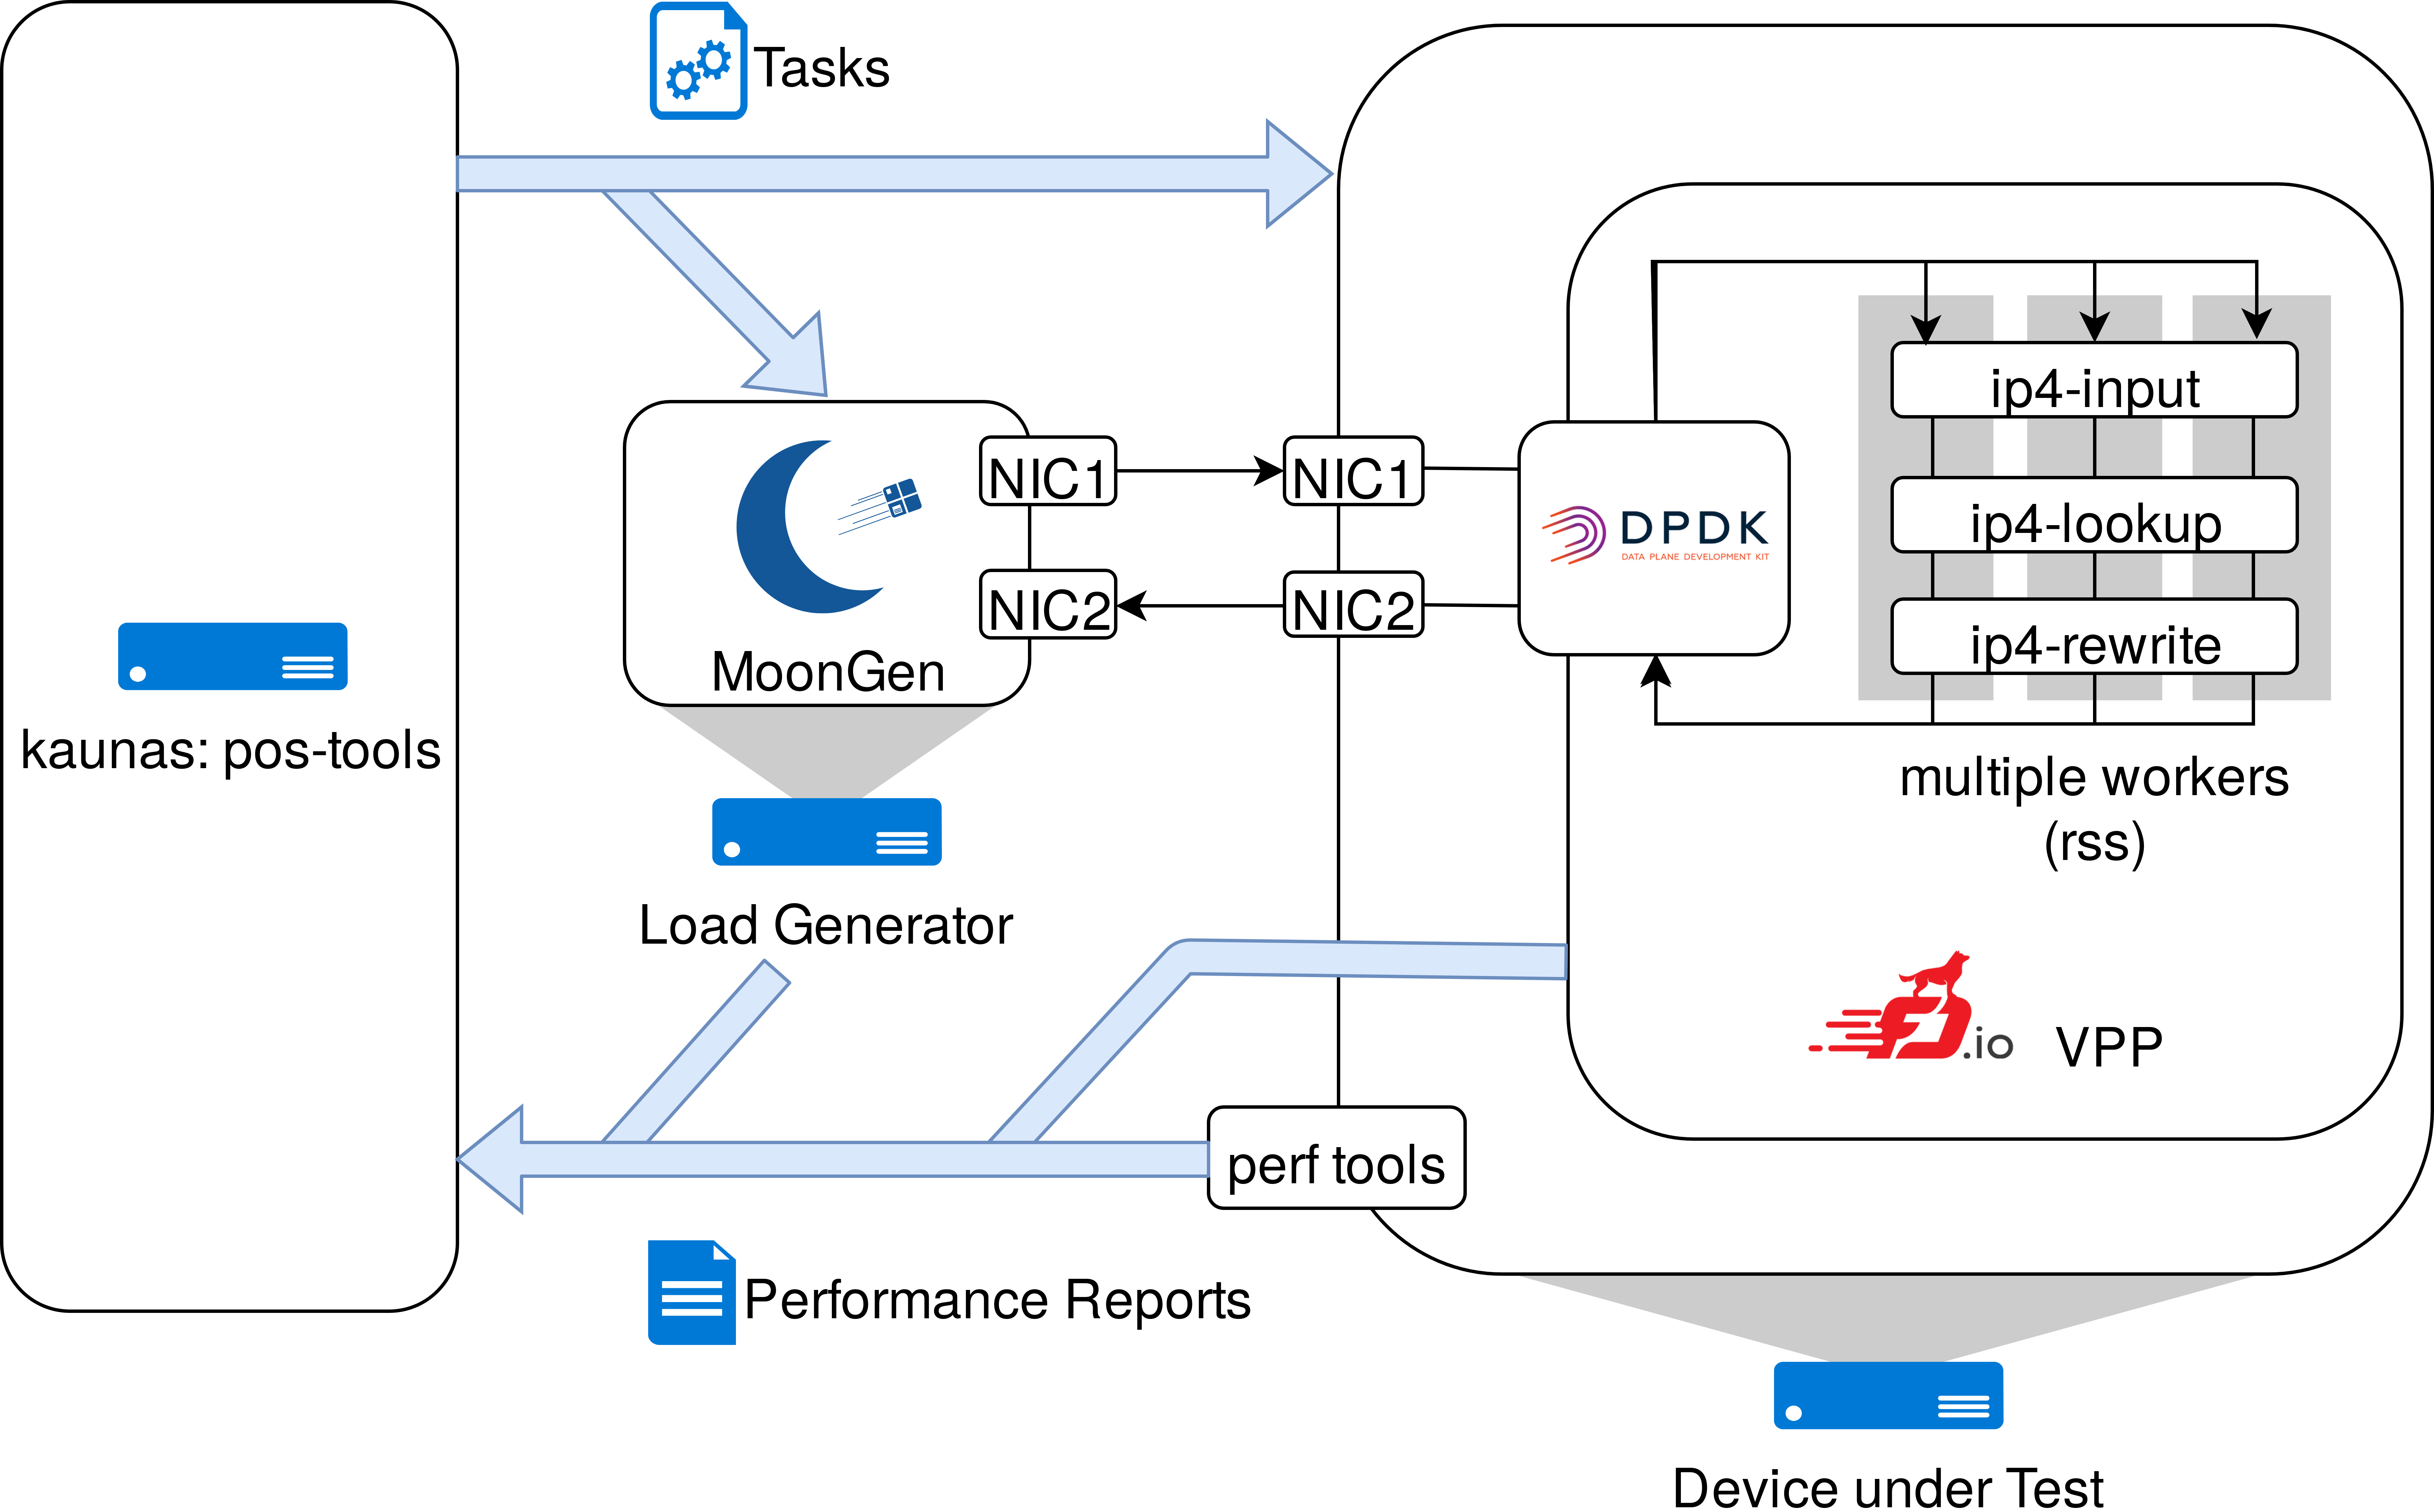
\includegraphics[width=\linewidth]{pics/topology.png}
\caption{Experiment setup for testing VPP with "kaunas" management server, loadgen and DUT}
\label{setup}
\end{figure}

\subsection{Performance Critical Parts}


\subsection{Packet Processing Graph}

% - modularity, feature rich
%	- visualize the parsing done in the first step as in the vpp paper and explain 
% 		bridging only: ip header parsing slowdown behaviour

 
\subsection{VPP's hash table implementations}


\subsection{Vectorization}

% - vectorization
% 	- low level optimization for caches
%	- more efficient instruction cache usage?
%	- VLIB_FRAME_SIZE


\subsection{NIC's with DPDK and VPP}

% - RSS
% - dpdk: fast userspace NIC drivers: busy polling mode


\subsection{experiment setup}


\subsection{Collected Data}

% why used testing methods: latency, throughput, perf/cache-misses

% Analyzes and assesses several possible approaches that solve the problem



